
\documentclass[12pt]{article}
 
\usepackage[margin=1in]{geometry} 
\usepackage{amsmath,amsthm,amssymb,enumitem,graphicx,verbatim,amsfonts,amscd,amsrefs}

\usepackage{hyperref}
\usepackage{setspace}
\usepackage{listings}

\newcommand{\N}{\mathbb{N}}
\newcommand{\Z}{\mathbb{Z}}
 
\newenvironment{theorem}[2][Theorem]{\begin{trivlist}
\item[\hskip \labelsep {\bfseries #1}\hskip \labelsep {\bfseries #2.}]}{\end{trivlist}}
\newenvironment{lemma}[2][Lemma]{\begin{trivlist}
\item[\hskip \labelsep {\bfseries #1}\hskip \labelsep {\bfseries #2.}]}{\end{trivlist}}
\newenvironment{exercise}[2][Exercise]{\begin{trivlist}
\item[\hskip \labelsep {\bfseries #1}\hskip \labelsep {\bfseries #2.}]}{\end{trivlist}}
\newenvironment{problem}[2][Problem]{\begin{trivlist}
\item[\hskip \labelsep {\bfseries #1}\hskip \labelsep {\bfseries #2.}]}{\end{trivlist}}
\newenvironment{question}[2][Question]{\begin{trivlist}
\item[\hskip \labelsep {\bfseries #1}\hskip \labelsep {\bfseries #2.}]}{\end{trivlist}}
\newenvironment{corollary}[2][Corollary]{\begin{trivlist}
\item[\hskip \labelsep {\bfseries #1}\hskip \labelsep {\bfseries #2.}]}{\end{trivlist}}
 
\begin{document}
 
 
\title{HW 1}
\author{Gabriella Mickel\\ 
STAT 5301} 
 
\maketitle
 
\begin{question}{1}
The file cbusairtemp.RData contains approximately 27 months of daily air temperature data for Columbus, Ohio. The air temperature measurements were made in degrees Farenheit.
\end{question}
 
\begin{enumerate}[label=(\alph*)]
\item Make a histogram of the data.

\begin{lstlisting}
> hist(air, breaks = "Scott", freq=F, main="", 
	xlab="Air Temperature (Farenheit)", col="grey"); 
	lines(density(air), col="red")
\end{lstlisting}

\begin{figure}[h!]
\centering
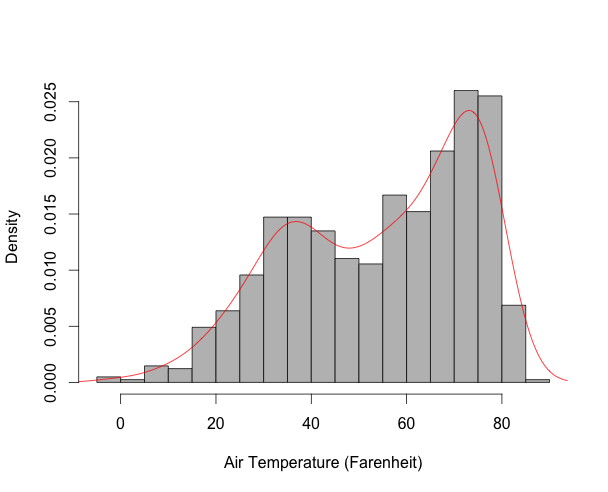
\includegraphics[scale = .6]{Rplot.png}
\end{figure}

\item Describe the shape, center and spread of the distribution based on the histogram.
-Shape: The histogram is bimodal. 

-Center: The center of the histogram is somewhere in the 50s. Quantitative description from R: mean = 54.91, mode =  75.6, median = 58.3.

-Spread: The data ranges from a little below zero to above 80 degrees Fahrenheit. Quantitative description from R: min = -1.8, 1st Qu. = 38.85, median = 58.30, mean = 54.91, 3rd Qu. = 72.10, max = 85.20, IQR = 33.25, range = 86.9, variance = 367.2307, standard deviation = 19.16326. 


\begin{lstlisting}
> getmode <- function(v) {
    uniqv <- unique(v)
    uniqv[which.max(tabulate(match(v, uniqv)))]
}
>getmode(air)
> sd(air); var(air); summary(air)
\end{lstlisting}


\item Make a time plot of the data. Do you notice any patterns? Do you notice any unusual observations?
\begin{lstlisting}
> plot.ts(air, xlab="Time (Days)", 
			ylab="Air Temperature (Degrees Farenheit)")
\end{lstlisting}

\begin{figure}[h!]
\centering
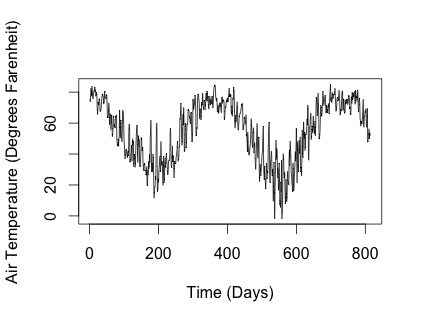
\includegraphics{timePlot.png}
\end{figure}

The time plot seems to repeat itself creating two similar u-like shapes. As this graph represents roughly two years (27 months), this repetition corresponds to two cycles through seasonal temperature changes in Columbus. The second winter was colder on average. 
\end{enumerate}


\begin{question}{2}
There is the stereotype that women are more talkative than men. A study examines this stereotype and collects data on the speech habits of 42 women and 37 men in the United States. In particular, the data set talk.RData records the number of words per day spoken by each individual in the study.
\end{question}

\begin{enumerate}[label=(\alph*)]
\item Make stemplots, separately, for the women and men. Describe and compare the shapes of the distributions.
\begin{lstlisting}
> with(talk, stem(WordsPerDay[GenderMale1 == "F"])); 
		with(talk, stem(WordsPerDay[GenderMale1 == "M"]))

 The decimal point is 4 digit(s) to the right of the |

  0 | 2
  0 | 5567888888899
  1 | 122244
  1 | 5566677777788
  2 | 0111224
  2 | 5
  3 | 2


  The decimal point is 4 digit(s) to the right of the |

  0 | 1223
  0 | 55577899
  1 | 0000011222
  1 | 56777
  2 | 24444
  2 | 67
  3 | 01
  3 | 6
  
\end{lstlisting}

Female has a bimodal distribution and less variance than male. Male has a right-skewed, unimodal distribution and more variance than female. 

\item Make side-by-side boxplots of the women and men. Are there any outliers for either group?
\begin{lstlisting}
> with(talk, boxplot(WordsPerDay ~ GenderMale1, 
				xlab = "Gender", 
				ylab = "Words per Day"))
\end{lstlisting}
\begin{figure}[h!]
\centering
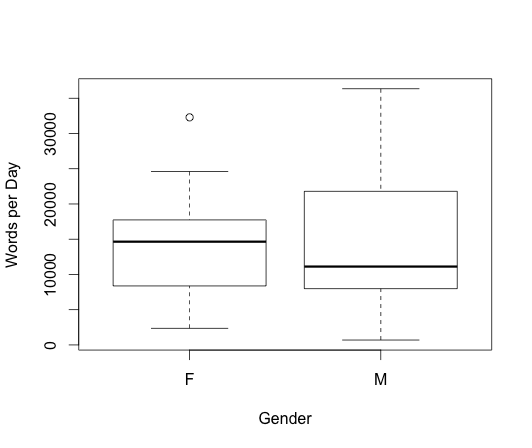
\includegraphics[scale=.8]{genderPlot.png}
\end{figure}
There is one outlier for the F group.  

\item Do you think that the data supports the stereotype? Explain your answer.

I do think the data leans slightly towards supporting the stereotype. This is because the medians suggest men talk less than women. The means suggest men and women talk about the same amount; however, means are sensitive to outliers, while medians are more resistant. 
\end{enumerate} 

\begin{question}{3}
The data set wineries.RData lists the year of founding of forty wineries in New Zealand.
\end{question}

\begin{enumerate}[label=(\alph*)]
\item Find the five-number summary for the data.
\begin{lstlisting}
> summary(wineries)
      Date     
 Min.   :1860  
 1st Qu.:1934  
 Median :1948  
 Mean   :1947  
 3rd Qu.:1975  
 Max.   :1983 
\end{lstlisting}

\item Make a boxplot of the data.
\begin{lstlisting}
> boxplot(wineries)
\end{lstlisting}

\begin{figure}[h!]
\centering
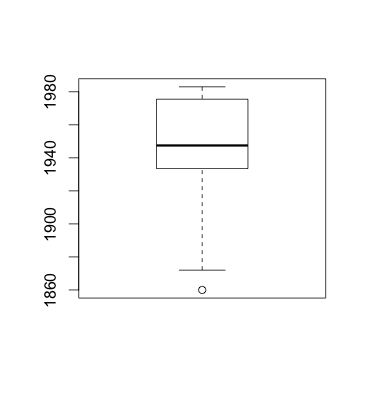
\includegraphics[scale=.8]{boxPlotWineries.png}
\end{figure}

\item Make three histograms of the data, each with different bin widths / numbers of breaks. (Try using the breaks= option in the R hist function.) Which bin width / number of breaks do you prefer?
\begin{lstlisting}
> hist(wineries$Date, breaks = 5)
> hist(wineries$Date, breaks = 2)
> hist(wineries$Date, breaks = 200)
\end{lstlisting}

\begin{figure}[h!]
\centering
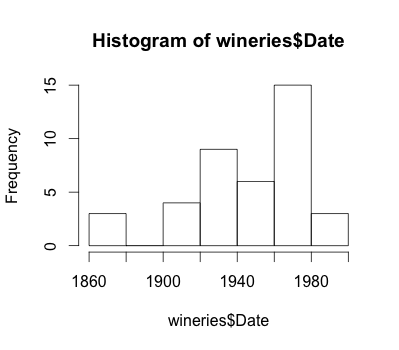
\includegraphics[scale=.8]{5.png}
\end{figure}
\begin{figure}[h!]
\centering
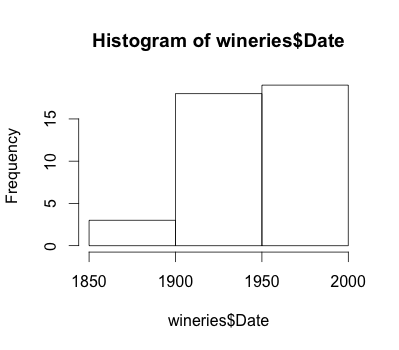
\includegraphics[scale=.8]{2.png}
\end{figure}
\clearpage
\begin{figure}[h!]
\centering
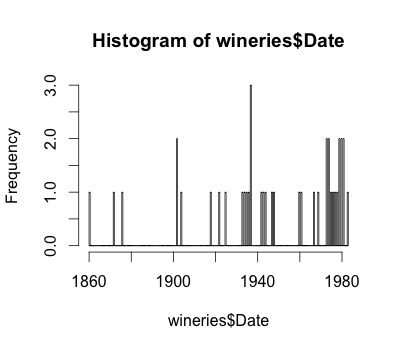
\includegraphics[scale=.8]{200.png}
\end{figure}

I prefer the breaks=5. With breaks=2 the information is overly summarized and all detail is lost. With breaks=200 the histogram is so detailed it is no longer a summary. 

\item Write a short summary of the major features of the distribution. Do you prefer the boxplot or the histogram for the data?

The distribution is bimodal. Center: mean= 1947, median= 1948, mode= 1937. Spread: range= 123, variance= 1088.285, standard deviation= 32.98916. I prefer the boxplot for the data because I can see frequency in more detail and have an easier time picturing the distribution. 
\end{enumerate}

\begin{question}{4}
The weights of Major League Baseball players follow a distribution that is approximately normal with mean 202 pounds and standard deviation 21 pounds. Use the 68-95-99.7 rule to answer the following questions.
\end{question}
\begin{enumerate}[label=(\alph*)]
\item Between what values are the middle 95 percent of player weights?

$(202-1.96(21), 202+1.96(21))=(160.84, 243.16)$
They are between 160.84 pounds and 243.16 pounds. 
\item Above what weight are the heaviest 2.5 percent of players?

They are above 243.16 pounds.
\item Below what weight are the lightest 16 percent of players?

$(202-21,202+21)=(181,223)$
They are below 181 pounds.
\end{enumerate}

 
% --------------------------------------------------------------
%     You don't have to mess with anything below this line.
% --------------------------------------------------------------
 
\end{document}